\documentclass[tikz,border=2mm]{standalone}
\definecolor{structure}{HTML}{1A535C}   % Deep Teal
\definecolor{main}{HTML}{C6892A}       % Golden Ochre
\definecolor{second}{HTML}{2E4057}     % Slate Blue
\definecolor{third}{HTML}{8B2635}      % Burgundy

\begin{document}

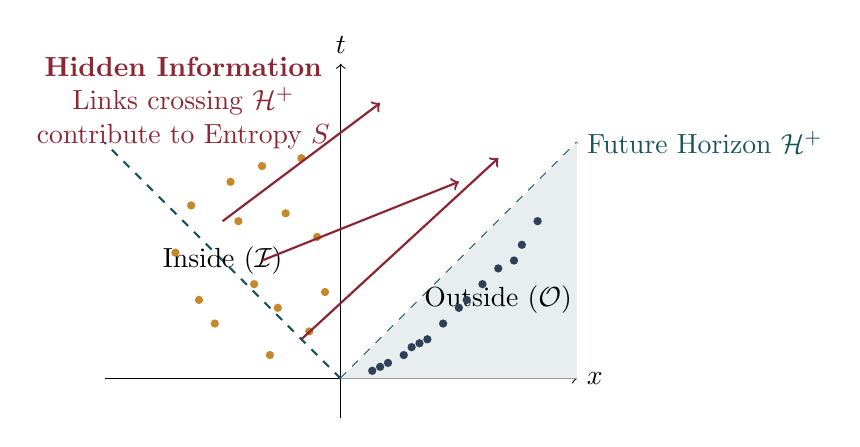
\begin{tikzpicture}[scale=1]

% ---- Axes and horizon ----
\draw[->] (-3,0) -- (3,0) node[right] {$x$};
\draw[->] (0,-0.5) -- (0,4) node[above] {$t$};

% Future lightcone (the horizon)
\draw[dashed, thick, color=structure]
    (0,0) -- (3,3) node[right] {Future Horizon $\mathcal{H}^+$};
\draw[dashed, thick, color=structure] (0,0) -- (-3,3);

% Rindler wedge shading
\fill[structure!10] (0,0) -- (3,3) -- (3,0) -- cycle;
\node at (2,1) {Outside ($\mathcal{O}$)};
\node at (-1.5,1.5) {Inside ($\mathcal{I}$)};

% ---- Sprinkled events (deterministic positions for reproducibility) ----
% Inside points (golden)
\foreach \px/\py in {
    -0.4/0.6, -1.1/1.2, -0.7/2.1, -1.8/1.0, -0.3/1.8,
    -1.4/2.5, -0.9/0.3, -2.1/1.6, -0.5/2.8, -1.6/0.7,
    -0.2/1.1, -1.3/2.0, -0.8/0.9, -1.0/2.7, -1.9/2.2
}{
    \fill[main] (\px,\py) circle (1.5pt);
}
% Outside points (slate)
\foreach \px/\py in {
    0.8/0.3, 1.5/0.9, 2.2/1.5, 0.4/0.1, 1.1/0.5,
    1.8/1.2, 2.5/2.0, 0.6/0.2, 1.3/0.7, 2.0/1.4,
    0.9/0.4, 1.6/1.0, 2.3/1.7, 0.5/0.15, 1.0/0.45
}{
    \fill[second] (\px,\py) circle (1.5pt);
}

% ---- Causal links crossing the horizon ----
\draw[->, color=third, thick] (-1, 1.5) -- (1.5, 2.5);
\draw[->, color=third, thick] (-0.5, 0.5) -- (2, 2.8);
\draw[->, color=third, thick] (-1.5, 2.0) -- (0.5, 3.5);

% Annotation
\node[align=center, color=third] at (-2, 3.5)
    {\textbf{Hidden Information} \\ Links crossing $\mathcal{H}^+$ \\
     contribute to Entropy $S$};

\end{tikzpicture}

\end{document}
